\documentclass{article}

\usepackage[utf8]{inputenc}
\usepackage{xeCJK}
\usepackage{kotex}
\usepackage{minted}
\usepackage{mdframed}
\usepackage{ntheorem}
\usepackage{fontspec}
\usepackage{color}
\usepackage{graphicx}
\usepackage[a4paper, top=15mm, bottom=15mm, left=20mm, right=20mm]{geometry}

\definecolor{codeblockbackground}{RGB}{245, 245, 245}
\definecolor{codeblockborder}{RGB}{200, 200, 200}

\theoremstyle{nonumberplain}
\newmintedfile[javacode]{java}{
  linenos=true,
  breaklines,
  fontfamily=D2Coding,
  framesep=2mm,
  bgcolor=codeblockbackground
}
\newminted[console]{text}{
  breaklines,
  fontfamily=D2Coding,
  framesep=2mm,
  bgcolor=codeblockbackground
}
\newmdtheoremenv[%
  backgroundcolor=codeblockbackground,
  linecolor=codeblockborder,
  outerlinewidth=3
]{code}{}

\graphicspath{ {./tex/} }

\title{자바프로그래밍및실습 과제 4}
\author{214823 컴퓨터정보통신공학과 박종현}
\date{May 2022}

\begin{document}

\maketitle
\pagebreak


코드 주석은 Javadoc 코드 문서화 스펙을 참조하여 작성함.

참조: https://docs.oracle.com/en/java/javase/17/docs/specs/javadoc/doc-comment-spec.html


\section{과제 1}
\subsection{소스코드}

\javacode{java/Prob1.java}

\subsection{실행 예제}
\subsubsection{예제 1}
\makebox{
  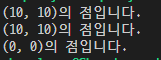
\includegraphics[width=\linewidth]{Prob1}
}



\section{과제 2}
\subsection{소스코드}

\javacode{java/Prob2.java}

\subsection{실행 예제}
\subsubsection{예제 1}
\makebox{
  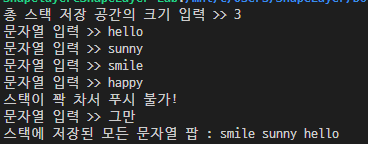
\includegraphics[width=\linewidth]{Prob2}
}



\section{과제 3}
\subsection{소스코드}

\javacode{java/Prob3/DictionaryApp.java}

\subsection{실행 예제}
\subsubsection{예제 1}
\makebox{
  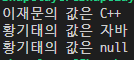
\includegraphics[width=\linewidth]{Prob3}
}



\section{과제 4}
\subsection{소스코드}

\javacode{java/Prob4.java}

\subsection{실행 예제}
\subsubsection{예제 1}
\makebox{
  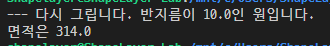
\includegraphics[width=\linewidth]{Prob4}
}



\section{과제 5}
\subsection{소스코드}

\javacode{java/Prob5.java}

\subsection{실행 예제}
\subsubsection{예제 1}
\makebox{
  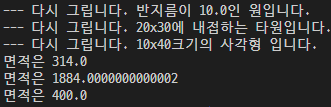
\includegraphics[width=\linewidth]{Prob5}
}




\end{document}
